\documentclass[output=paper]{LSP/langsci}  
\author{Simonetta Montemagni\affiliation{Istituto di Linguistica Computazionale “Antonio Zampolli”, ILC-CNR} \lastand Martijn Wieling\affiliation{University of Groningen, CLCG}} 
\title{Tracking linguistic features underlying lexical variation patterns: {A} case study on {T}uscan dialects} 
\rohead{\thechapter\hspace{.5em} Tracking linguistic features underlying lexical variation patterns}
\abstract{In this paper, we illustrate the application of hierarchical spectral partitioning of bipartite graphs in the study of lexical variation in Tuscany based on the data from a regional linguistic atlas. This method makes it possible not only to identify existing patterns of lexical variation in Tuscany, but also to uncover the underlying \isi{lexical features} in terms of the most characteristic concept-lexicalization pairs. The results are promising, demonstrating the potential of the method for tracking the linguistic features underlying identified patterns of lexical variation and change across generations.
}

\ChapterDOI{10.17169/langsci.b81.86 }
\maketitle 
\begin{document}
 
 
% 
% Tracking linguistic features underlying lexical variation patterns: A case study on \il{Italian!Tuscan}Tuscan dialects
% \vskip11pt

% \begin{multicols}{2}
% Simonetta Montemagni\\
% 
% 
% Martijn Wieling\\
% 
% \end{multicols}
% 
% \begin{abstract}
% .
% \end{abstract}

\section{Introduction}
In dialectometry \citep{seguy_relation_1971} the focus lies on the aggregate analysis of dialect variation. In contrast to “cherry-picking” a few linguistic items confirming the analysis one wishes to settle on \citep{nerbonne_data-driven_2009}, the advantage of the aggregate approach is that it offers a more objective view of dialect variation. Unfortunately, many studies focusing on the aggregate pattern of dialect variation have disregarded the underlying linguistic basis. As a consequence, linguists have remained critical of the dialectometric approach \citep{schneider_qualitative_1988,woolhiser_political_2005, loporcaro_profilo_2009}. 

To counter this criticism, various new dialectometric methods have been developed aimed at identifying the linguistic basis of dialectal variation (as reviewed in \citealt{wieling_advances_2015}). For example, \citet{nerbonne_identifying_2006} and \citet{proll_latente_inpress} use an approach based on factor analysis, whereas \citet{shackleton_english-american_2005} uses principal component analysis. \citet{grieve_statistical_2011} follow the workflow of traditional dialectology (i.e. identifying isoglosses, bundling isoglosses and cluster analysis) by using multivariate spatial analysis. 

The method we will apply here, Hierarchical Bipartite Spectral Graph Partitioning (HBSGP)\is{hierarchical bipartite spectral graph partitioning}, has been developed by \citet{wieling_bipartite_2009,wieling_hierarchical_2010, wieling_bipartite_2011}, who adopted it from information retrieval \citep{dhillon_co-clustering_2001} and applied it to dialectology. HBSGP results in a clustering\is{dialect clustering} of geographical varieties while \emph{simultaneously }providing a linguistic basis for each of the identified clusters. The approach of \citet{wieling_bipartite_2011} has been successfully applied to study phonetic variation in \ili{Dutch} dialects \citep{wieling_bipartite_2011}, English dialects \citep{wieling_analyzing_2013} and \il{Italian!Tuscan}Tuscan dialects \citep{montemagni_patterns_2012,montemagni_synchronic_2013}. More recently, the method has also been applied to investigate \isi{lexical variation} in contemporary English dialects on the basis of the BBC \textit{Voices} data \citep{wieling_lexical_2014}.

In this study, we focus on lexical variation. Our dataset, a regional lexical atlas of \il{Italian!Tuscan}Tuscan dialects whose data have a diatopic and diachronic characterization, allows us to explore the potential of the HBSGP method in the study of \isi{lexical variation}. In particular, it enables us to identify \isi{lexical features} and their relationships on the one hand and to reconstruct the dynamics of \isi{lexical change} across generations on the other hand. Technically, a new measure is proposed for determining the most important \isi{lexical features} associated with the identified dialectal areas.

\section{Data}
We investigate \il{Italian!Tuscan}Tuscan lexical variation on the basis of a linguistic atlas of Tuscany, the \textit{Atlante Lessicale Toscano} (ALT, \citealt{giacomelli_atlante_2000}), now available as an online resource (\url{http://serverdbt.ilc.cnr.it/ALTWEB}). ALT is a regional Italian lexical atlas focusing on dialectal variation throughout Tuscany, where both \il{Italian!Tuscan}Tuscan and non-\il{Italian!Tuscan}Tuscan dialects are spoken. In this paper we focus on \il{Italian!Tuscan}Tuscan dialects only, recorded in 213 localities by a total of 2060 informants who were selected with respect to various socio-demographic parameters (such as age, education and gender). 

ALT interviews were carried out on the basis of a questionnaire of 745 target items, designed to elicit mainly lexical, but also semantic and phonetic variation. This study is based on the results of onomasiological questions, i.e. starting from concepts and looking for their lexicalizations. A typical onomasiological question asks how a given concept is designated or named, e.g. “what is the name for flat and crispy bread, seasoned with salt and oil?”. To avoid interference with non-lexicalized answers, we excluded questions prompting 50 or more distinct lexical items. Furthermore, we only considered nouns (the large majority of items of ALT questionnaire) in this study. The resulting subset consists of 170 questionnaire items for which a total of 5,174 distinct normalized answers were given (on average 30 lexical variants per concept) distributed into 61,496 geo-referenced responses (i.e. associated with locations). The total number of speaker-responses was 384,454. 

To abstract away from phonetic variation, we used the most abstract representation level present in ALT \citep{cucurullo_dialectal_2006}. This normalized representation was meant to abstract from phonetic variation (caused by productive phonetic processes), but did not remove morphological variation or variation caused by unproductive phonetic processes. In this study we used the normalized lexical answers to the selected subset of 170 onomasiological questions. The same set of questions has also been used by \citet{wieling_analyzing_2014} in a study of lexical differences between \il{Italian!Tuscan}Tuscan dialects and standard Italian.

The \isi{representativeness} of the selected sample with respect to the whole set of ALT onomasiological questions (i.e. a total of 460 questionnaire items) was assayed using the correlation between overall lexical distances and lexical distances obtained from the selected sample \citep{wieling_analyzing_2014}. The Pearson’s correlation coefficient was \textit{r} = 0.94, showing the \isi{representativeness} of the selected sample with respect to the whole set of onomasiological questions.

\section{Methods}
In this study, we use \isi{hierarchical bipartite spectral graph partitioning} as our method of choice (\cite{wieling_bipartite_2011}). As mentioned before, this approach simultaneously clusters the geographic locations together with the linguistic features characterizing them. In this case, a cluster of locations is characterized by a linguistic basis expressed in terms of the most salient \isi{lexical features}. These \isi{lexical features} can be seen as a proxy of the traditional notion of lexical isoglosses, establishing the boundaries of dialectal areas.

Every variety attested in a given location is described in terms of Concept-Lexicalization (CL) pairs\is{concept-lexicalization pair} linking each of the 170 selected concepts with its lexicalization(s) (reported in the normalized form) in the specific location. CL frequencies are normalized by dividing the number of recorded answers by the number of informants in a given location, with their value ranging between 0 and 1. Since there was a socio-demographically differentiated group of informants potentially giving rise to multiple responses to denote the same concept for each location, the sum of normalized frequencies of lexical variants associated with the same concept in a certain location can be greater than 1.

The input for the HBSGP method is a bipartite graph which contains two sets of vertices, locations and CL pairs, connected by lines. There exists a line between a location and a CL pair whenever at least one of the speakers in the location uses the lexical variant. The lines are weighted between 0 and 1. A value of~0 indicates that no speakers in the location use the lexical variant (and thus equals the absence of a line), whereas a value of~1 indicates that all speakers in the location use the lexical variant to denote the concept being investigated. \tabref{tab:monte:1} gives an example of (a tabular representation of) the bipartite graph, with the rows corresponding to the locations and the columns to the CL pairs. About 80\% of the speakers in Caprese Michelangelo use the form \textit{aràncio} to denote an \textsc{orange} (henceforth, concept denominations are represented by small caps). A similar number of speakers also uses \textit{melàngola} to denote the same (speakers frequently provided multiple lexicalizations to denote a certain concept). 

The input matrix is then subjected to Singular Value Decomposition \is{singular value decomposition} (SVD), and the \is{k-means clustering@\textit{k}-means clustering}\textit{k}-means clustering\is{dialect clustering} algorithm (with \textit{k} equals 2) is applied to the results of the SVD resulting in a two-way clustering. The \textit{k}{}-means clustering was repeated 1000 times for robustness. As the output of the SVD combines the locations with the CL pairs, the clustering\is{dialect clustering} likewise groups locations and CL pairs. Consequently, lexical variants grouped with locations can be seen as characteristic elements of those locations. For more mathematical details, we refer the interested reader to \citet{wieling_bipartite_2011}. 

\begin{table}
\resizebox{\textwidth}{!}{
\begin{tabular}{llll}
\lsptoprule
%{\bfseries Location} & {\bfseries \textsc{orange}{}-\textit{arància}} & {\bfseries \textsc{orange}{}-\textit{aràncio}} & {\bfseries \textsc{orange}{}-\textit{melàngola}}\\
{ Location} & { \textsc{orange}{}-\textit{arància}} & { \textsc{orange}{}-\textit{aràncio}} & { \textsc{orange}{}-\textit{melàngola}}\\
\midrule
{ Caprese Michelangelo} & 0.1379 & 0.7931 & 0.7931\\
{ Pieve Santo Stefano} & 0.4000 & 0.7333 & 0.2000\\
{ Anghiari} & 0.0000 & 0.7059 & 1.0000\\
{ Sansepolcro} & 0.0000 & 1.0000 & 1.0000\\
\lspbottomrule
\end{tabular}
}
\caption{Tabular representation of a bipartite graph. The numbers represent the normalized frequency (obtained by dividing by the number of speakers) of the lexical variant associated with a given concept in the different locations which ranges between 0 and 1. As the speakers may use multiple variants to denote a concept, the normalized frequencies associated with a concept in a certain location do not have to sum to 1.}
\label{tab:monte:1}
\end{table}

In order to identify the most characteristic linguistic features for a group of locations, \citet{wieling_bipartite_2011} combined two different criteria which were implemented in two different and complementary measures: \isi{representativeness} and distinctiveness.\is{distinctiveness|(} Representativeness measures the relative frequency of the lexicalization of a given concept in the locations in the cluster. For example, if the cluster contains ten locations and all speakers in seven locations use the lexical variant, the \isi{representativeness} is 0.7. Distinctiveness measures how frequently the lexical variant occurs within as opposed to outside of the cluster (corrected for the relative size of the cluster, which is calculated by dividing the number of locations in the cluster by the total number of locations in the dataset). A distinctiveness of 1 indicates that the lexical variant is only used inside the cluster. The distinctiveness equals 0 when the relative frequency of the lexical variant in the cluster is equal to the relative size of the cluster (i.e. it is not distinctive). Interestingly, the measures of \isi{representativeness} and distinctiveness are reminiscent of the “consistency” and “homogeneity” measures introduced by Labov and colleagues for the construction of isoglosses in the \textit{Atlas of North American English} \citep{labov_atlas_2006-1}. Homogeneity measures how much variation exists within the region defined by the isogloss (i.e. corresponding to a non-chance corrected variant of distinctiveness) and consistency (i.e. corresponding to \isi{representativeness}) measures how strongly the variable is concentrated within a given region.

The two measures capture two different equally important desiderata of isoglosses: to put it in the words of \citet{labov_atlas_2006-1}, “First, we want the area defined to be as uniform as possible […]. Second, we want as high a proportion of hits as possible to be located within the isogloss”. For this reason they need to be combined. \citet{wieling_bipartite_2011} combined \isi{representativeness} and distinctiveness\is{distinctiveness|)} measures by averaging them, yielding the \isi{importance} score. Here, we propose that to determine the relevance of CL pairs in the characterization of identified lexical areas\is{lexical area} it is better to multiply the two values. The advantage of this approach is that it is not possible to assign high \isi{importance} values to lexical variants which score high on a single measure only. For example, lexical variants occurring in all locations are highly representative, but not distinctive. Similarly, a lexical variant only occurring in a single location is highly distinctive, but not representative (unless the cluster contains a single location). Note that constraints on isogloss construction were also foreseen by \citet{labov_atlas_2006-1} by enforcing frequency thresholds. However, the advantage of the approach proposed by \citet{wieling_bipartite_2011} and its evolution presented here consists in the fact that no \textit{a priori} constraints on the values of individual measures are defined.

\section{Results}
In this section, we report the results of applying the HBSGP method to the selected ALT dataset. The results obtained are based on 5,174 CL pairs and 213 locations, which correspond to all lexical data gathered through fieldwork (as opposed to a dataset in which infrequent lexical variants are filtered out) for the 170 selected concepts. See \citet{wieling_infrequent_2015} for a discussion of the advantages connected with this dataset. 

\begin{figure}[b]
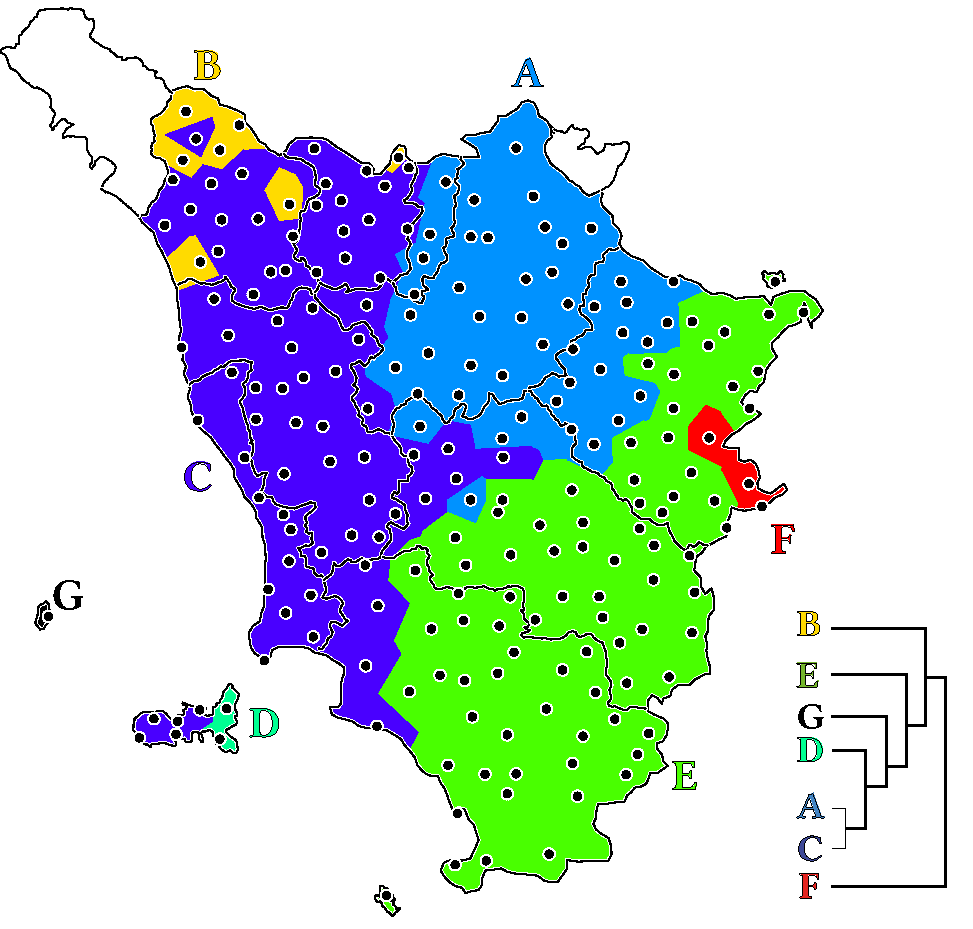
\includegraphics[width=.8\textwidth]{illustrations/monte_wiel_fig1_v2} 
\caption{Geographic visualization of the clustering of \il{Italian!Tuscan}Tuscan varieties into seven groups.} 
\label{fig:monte:1}
\end{figure}

The map in \figref{fig:monte:1} shows the geographic visualization of the clustering of \il{Italian!Tuscan}Tuscan varieties into seven groups designated as follows: the Florence area (A), the western \il{Italian!Tuscan}Tuscan area (C) and the dialects from Arezzo, Siena, Grosseto and Mount Amiata (E) which represent the three main groupings, together with the dialects from Elba island (D), Chiana Valley (F), Capraia Island (G) and Apuan Alps (B) which are minor but clearly distinct dialectal areas.



It is interesting to note that this result is in line with the classifications of \il{Italian!Tuscan}Tuscan dialects proposed by \citet{giacomelli_aree_1975} for what concerns the lexicon, and by \citet{giannelli_toscana_1976} which is based instead on phonetic, phonemic, morpho-syntactic and \isi{lexical features}. It is also in line with the subdivision of \il{Italian!Tuscan}Tuscan dialects by \citet{pellegrini_carta_1977}, in spite of it being mainly based on the distribution of phonetic phenomena.

\subsection{Linguistic features underlying identified lexical areas}

For what concerns the underlying \isi{lexical features}, we first focus on the three main dialectal clusters (A, C and E). \tabref{tab:monte:2} reports for each cluster the five most important CL pairs with associated values of \isi{representativeness}, \isi{distinctiveness} and \isi{importance}.
 
\begin{table}[b]
\resizebox{\textwidth}{!}{
\begin{tabular}{p{1.5cm}lrrr}
\lsptoprule
Cluster & Concept-Lexicalization pair & Representativeness & Distinctiveness & Importance\\
\midrule
E 	& \textsc{turkey}-\emph{bìllo} 				&  0.863 & 0.700 & 0.604\\
	& \textsc{corner of tissue}-\emph{pìnzo} 	&  0.724 & 0.795 & 0.576\\
	& \textsc{eye gum}-\emph{cipìcchia} 		&  0.624 & 0.920 & 0.574\\
	& \textsc{oil jar}-\emph{zìro} 				&  0.879 & 0.609 & 0.535\\
	& \textsc{vat}-\emph{bigónzo} 				&  0.649 & 0.821 & 0.533\\
\midrule
A	& \textsc{orange}-\emph{arància} 			&  0.779 & 0.675 & 0.526\\
	& \textsc{ladle}-\emph{romaiòlo} 			&  0.788 & 0.536 & 0.423\\
	& \textsc{oil jar}-\emph{órcio} 			&  0.671 & 0.590 & 0.396\\
	& \textsc{turkey}-\emph{tàcco} 				&  0.390 & 1.000 & 0.390\\
	& \textsc{brawn}-\emph{capofréddo} 			&  0.432 & 0.900 & 0.389\\
\midrule
C 	& \textsc{oil jar}-\emph{cóppo} 			&  0.749 & 0.696 & 0.522\\
	& \textsc{eye gum}-\emph{cìspia} 			&  0.702 & 0.676 & 0.474\\
	& \textsc{breast}-\emph{pùppa} 				&  0.649 & 0.717 & 0.466\\
	& \textsc{flea}-\emph{pùce} 				&  0.602 & 0.686 & 0.413\\
	& \textsc{cluster of grapes}-\emph{pìgna} 	&  0.570 & 0.701 & 0.400\\
\lspbottomrule
\end{tabular}
}
\caption{The five topmost lexical variants for the three main clusters of \il{Italian!Tuscan}Tuscan dialects.}
\label{tab:monte:2}
\end{table}

 
The relevance of the \isi{lexical features} with respect to the dialectal subdivision emerges clearly from the value maps in \figref{fig:monte:2}, which show the geographic distribution of the first and second topmost \isi{lexical features} of each of the three main identified clusters (A, C and E). The topmost \isi{lexical features} associated with each identified cluster can be assimilated with the traditional notion of \isi{bundle of isoglosses}, which have long been considered a major criterion for the definition of dialect areas: as \citet{chambers_dialectology_1998} put it, “the significance of a dialect area increases as more and more isoglosses\is{isogloss} are found which separate it from adjoining areas”.



\begin{figure}[t]
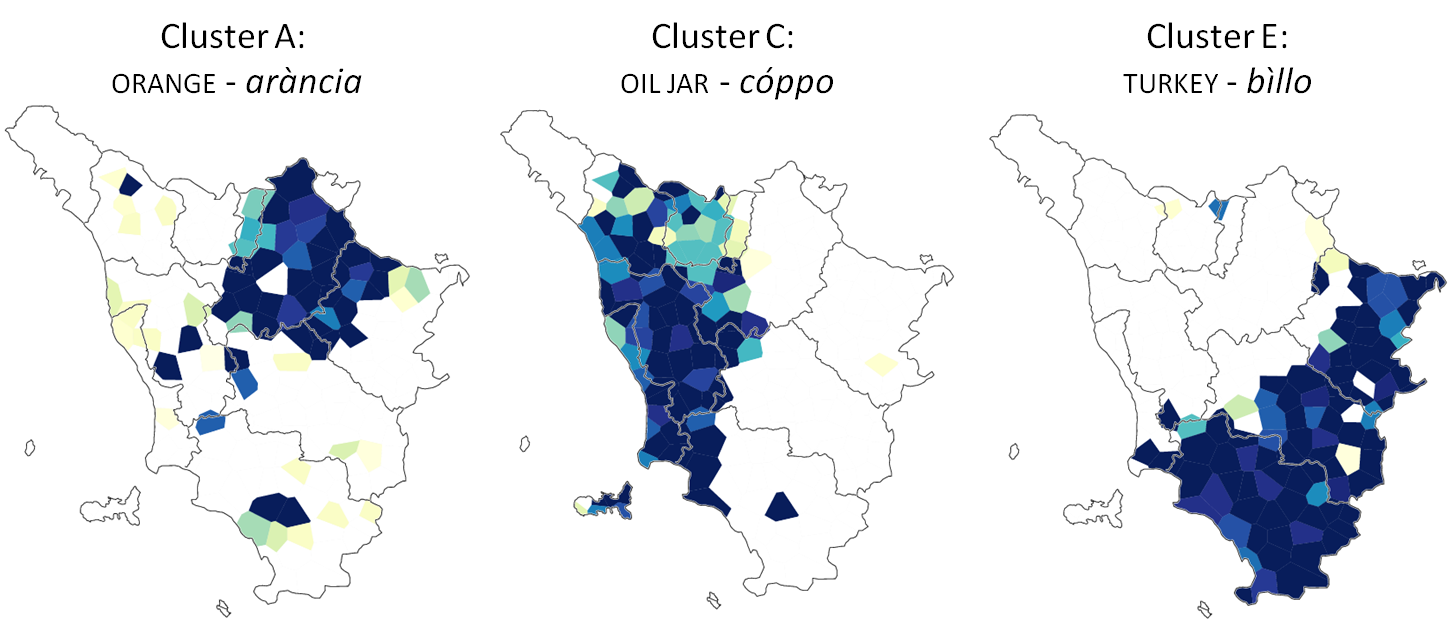
\includegraphics[width=\textwidth]{illustrations/monte_wiel_fig21}\\
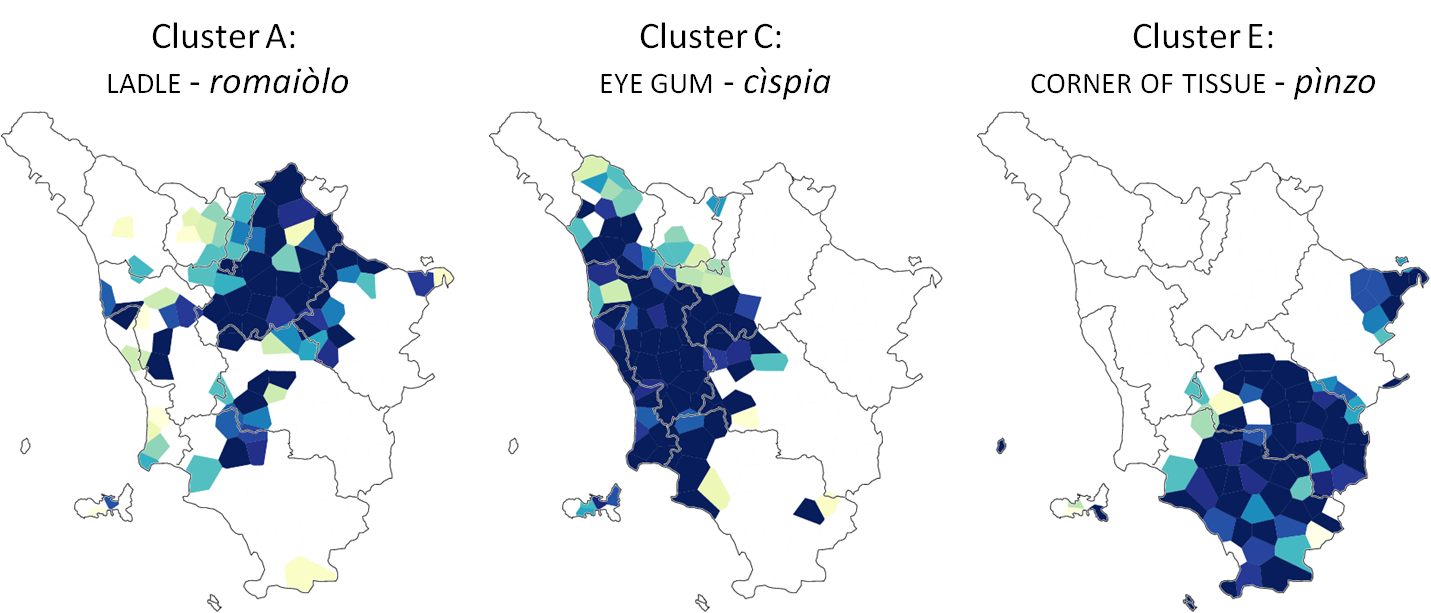
\includegraphics[width=\textwidth]{illustrations/monte_wiel_fig22} 
\caption{Value maps of the first (row 1) and second (row 2) topmost CL pairs for the A, C and E dialectal clusters. Areas with darker (blue) color denote a greater frequency of occurrence of the selected lexical variant; lighter colors denote a lower frequency, while no coloring (white) denotes the absence of the variant.}
\label{fig:monte:2}
\end{figure}

By comparing the maps of \figref{fig:monte:2}, we can observe that the geographic distribution of the topmost CL pairs of the E, A and C clusters does not cover all and only the locations in the cluster. Each of them can be seen as a quantitative visualization of individual isoglosses\is{isogloss}, where darkness of color denotes the frequency of occurrence of the represented lexical variant (dark colors denote a greater frequency, lighter colors lower frequency, and no coloring indicates the absence of the variant). As can be observed, lexical variants shown in \tabref{tab:monte:2} may occur beyond the border of the cluster area, thus lowering the distinctiveness \is{distinctiveness|(} value of the CL pair, or they may not occur in the whole cluster area resulting in a lower representativeness. For instance, in cluster A comparable representativeness values are observed for the two topmost CL pairs (0.77-0.78), whereas the CL ranked in second place, i.e. \textsc{ladle}{}-\textit{romaiòlo}, has a lower distinctiveness value (0.53) than the topmost CL (i.e. whose distinctiveness value is 0.67). Different patterns can be observed in clusters E and C, with decreasing representativeness and increasing distinctiveness in the former case, and with both of them decreasing in the latter case. Despite these slight differences, in all cases representativeness and distinctiveness show relatively high values which never reach the value of~1 (with the only exception of the CL pair \textsc{turkey}{}-\textit{tàcco} in cluster A whose distinctiveness is equal to 1). The average values of the five topmost \isi{lexical features} for \isi{representativeness} and distinctiveness range between 0.61 and 0.74, and 0.69 and 0.77 respectively, demonstrating that the corresponding dialect areas are not marked by very clear and strong dialect borders\is{dialect border}. 

\begin{table}[p]
\resizebox{\textwidth}{!}{
\begin{tabular}{p{1.5cm}lrrr}
\lsptoprule
{ Cluster} & { Concept-Lexicalization pair} &  { Representativeness} &  { Distinctiveness} &  { Importance}\\
\midrule
{ F} & { \textstylehps{\textsc{finch}}{}-\textit{frenguéllo}} &  1.000 &  1.000 &  1.000\\
& { \textstylehps{\textsc{cucumber}}{}-\textit{citróne}} &  1.000 &  0.973 &  0.973\\
& { \textstylehps{\textsc{hail}}{}-\textit{granìschia}} &  0.667 &  1.000 &  0.667\\
& { \textstylehps{\textsc{goose}}{}-\textit{ciucióne}} &  0.667 &  1.000 &  0.667\\
& { \textstylehps{\textsc{lizard}}{}-\textit{racanàccio}} &  0.667 &  1.000 &  0.667\\
\midrule
{ B} & { \textstylehps{\textsc{snow}}\textstyleatn{{}-}\textit{gnéva}} &  0.429 &  1.000 &  0.429\\
& { \textstylehps{\textsc{rolling pin}}\textstyleatn{{}-}\textit{canèlla}\textstyleBookTitle{\textmd{ }}} &  0.429 &  1.000 &  0.429\\
& { \textstylehps{\textsc{stye}}\textstylehps{{}-}\textit{orzaiolo}\textstyleBookTitle{\textmd{ }}} &  0.653 &  0.633 &  0.414\\
& { \textstylehps{\textsc{garbage}}\textstyleatn{{}-}\textit{rùsco}\textstyleBookTitle{\textmd{ }}} &  0.531 &  0.734 &  0.389\\
& { \textstylehps{\textsc{lizard}}\textstyleatn{{}-}\textit{ciortellóne}} &  0.430 &  0.853 &  0.367\\
\midrule
{ D} & { \textstylehps{\textsc{hornet-}}\textit{buffóne}\textstyleBookTitle{\textmd{\textup{ }}}} &  0.950 &  1.000 &  0.950\\
& { \textstylehps{\textsc{khakis}}\textstyleBookTitle{\textmd{\textup{{}-}}}\textit{cicàchi}} &  0.500 &  1.000 &  0.500\\
& { \textstylehps{\textsc{khakis}}\textstyleBookTitle{\textmd{\textup{{}-}}}\textit{cicàco}} &  0.500 &  1.000 &  0.500\\
& { \textstylehps{\textsc{pine cone}}\textstyleBookTitle{\textmd{\textup{{}-}}}\textit{pignòcca}\textstyleBookTitle{\textmd{\textup{ }}}} &  0.500 &  1.000 &  0.500\\
& { \textstylehps{\textsc{trough-}}\textit{tròlego}\textstyleBookTitle{\textmd{\textup{ }}}} &  0.500 &  1.000 &  0.500\\
\midrule
{ G} & { \textstyleBookTitle{\textsc{watermelon}}{}-\textit{patècca}\textstyleBookTitle{\textmd{ }}} &  1.000 &  1.000 &  1.000\\
& { \textstyleBookTitle{\textsc{melon}}{}-\textit{melòne}} &  1.000 &  1.000 &  1.000\\
& { \textstyleBookTitle{\textsc{cluster}}{}-\textit{raspòllo}\textstyleBookTitle{\textmd{ }}} &  1.000 &  1.000 &  1.000\\
& { \textstyleBookTitle{\textsc{squirrel}}{}-\textit{miseràngolo}\textstyleBookTitle{\textmd{ }}} &  1.000 &  1.000 &  1.000\\
& { \textstyleBookTitle{\textsc{lizard-}}\textit{bìscia}\textstyleBookTitle{\textmd{ }}} &  1.000 &  1.000 &  1.000\\
\lspbottomrule
\end{tabular}
}
\caption{The five topmost lexical variants for the smaller peripheral areas F, B, D and G.}
\label{tab:monte:3}
\end{table}

\begin{figure}[p]
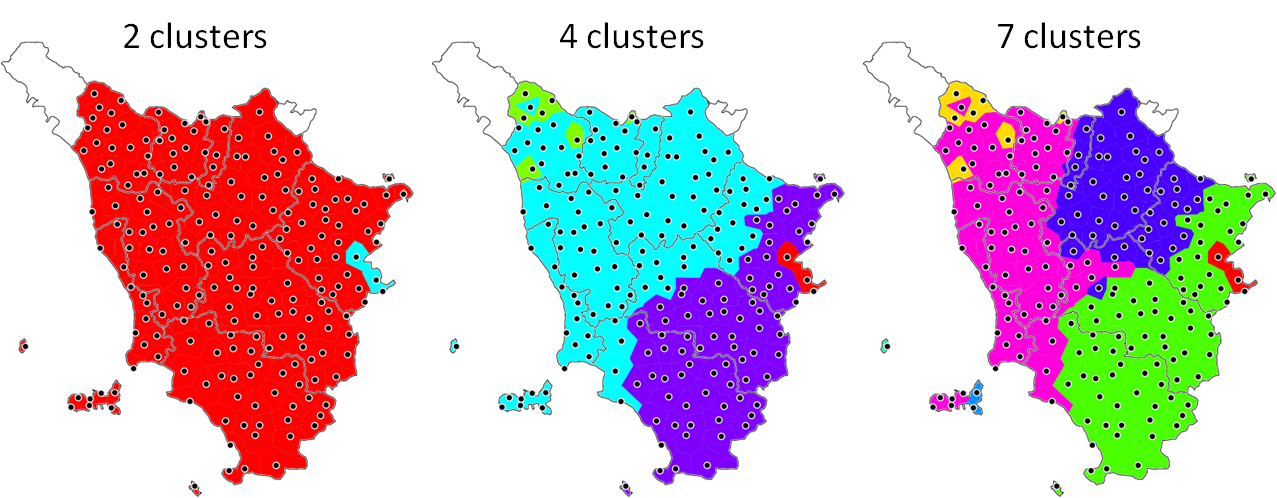
\includegraphics[width=\textwidth]{illustrations/monte_wiel_fig3} 
\caption{Geographic visualization of the clustering of \il{Italian!Tuscan}Tuscan varieties into two, four and seven groups.}
\label{fig:monte:3}\is{dialect clustering}
\end{figure}


Different distinctiveness-representativeness patterns are observed in the case of the smaller peripheral areas B, D, F and G (see \tabref{tab:monte:3}). Here, the most salient CL pairs are highly distinctive (their average values ranges from 0.84 to 1), with the average \isi{representativeness} ranging from 0.49 to 1. Thus smaller dialect areas are characterized by much more distinctive features than the larger areas.\is{distinctiveness|)}

Besides the strength of dialectal borders\is{dialect border}, granularity of the identified dialectal areas is another open issue in the study of dialectal variation. Consider, for instance, the traditional dialectal subdivision of \il{Italian!Tuscan}Tuscan dialects by \citet{pellegrini_carta_1977} and \citet{giannelli_toscana_1976}. In his \textit{Carta dei Dialetti d’Italia, }\citet{pellegrini_carta_1977} identifies a western variety of \il{Italian!Tuscan}Tuscan which is further subdivided into Pisano-Livornese-Elbano, and Pistoiese and Lucchese. On the other hand, \citet{giannelli_toscana_1976} identifies Pisano-Livornese, Lucchese, Elbano and Pistoiese as independent dialectal varieties in his seminal work \textit{Toscana}. The two subdivisions are compatible with each other but adopt different levels of granularity\is{granularity of dialectal areas}, i.e. they are seen through lenses differing in their magnifying power. Depending on the specific goals of a study, different levels of granularity of the dialectal landscape may be appropriate. By exploiting the hierarchical clustering\is{dialect clustering} results, the HBSGP method can also be used to identify increasingly smaller dialectal areas associated with progressively more specific \isi{lexical features}. These nested dialect areas are characterized by \isi{nested isoglosses} (i.e. the spatial distribution of one feature is entirely contained within that of another). To assess these \isi{nested isoglosses}\is{isogloss}, we compare the geographical and linguistic results obtained by clustering the selected dataset into two, four and seven groups (with the latter representing the clustering discussed so far).
 

\figref{fig:monte:3} reports the geographic visualization of clustering\is{dialect clustering} the \il{Italian!Tuscan}Tuscan varieties into two, four and seven groups. In the map with two clusters (\figref{fig:monte:3}, left), the large red cluster corresponds to the composite set of \il{Italian!Tuscan}Tuscan dialects, excluding only the Chiana Valley dialects (cyan cluster). The map with four clusters (\figref{fig:monte:3}, middle) shows the main subdivision of \il{Italian!Tuscan}Tuscan dialects between Northern dialects (cyan and green clusters), covering (from east to west) Fiorentino, Pistoiese, Lucchese and Pisano-Livornese, and Southern dialects (violet and red clusters), i.e. (from east to west) the dialect from Arezzo, Siena and Grosseto (violet cluster) and from the Chiana valley (red cluster). The map containing seven clusters (\figref{fig:monte:3}, right) has already been discussed above. 


\begin{table}[t]
\resizebox{\textwidth}{!}{
\begin{tabular}{p{1.5cm}lrrr}
\lsptoprule
{ Cluster} & { Concept-Lexicalization pair} &  { Representativeness} &  { Distinctiveness} &  { Importance}\\
\midrule
\multirow{4}{*}{\parbox{1.5cm}{Two-cluster map: Red}}
& \textstyleBookTitle{\textsc{sink}}\textstyleBookTitle{{}-}\emph{acquàio} &  0.909 &  1.000 &  0.909\\
& { \textstyleBookTitle{\textsc{celery}}\textstyleBookTitle{{}-}\emph{sèdano}} &  0.853 &  1.000 &  0.853\\
& { \textstyleBookTitle{\textsc{melon}}\textstyleBookTitle{{}-}\emph{popóne}} &  0.844 &  1.000 &  0.844\\
& { \textstyleBookTitle{\textsc{laurel}}\textstyleBookTitle{{}-}\emph{allòro}} &  0.801 &  1.000 &  0.801\\
& { \textstyleBookTitle{\textsc{watermelon}}\textstyleBookTitle{{}-}\emph{cocómero}} &  0.794 &  1.000 &  0.794\\
\midrule
\multirow{4}{*}{\parbox{1.5cm}{Four-cluster map:  Cyan}} 
& { \textstyleBookTitle{\textsc{thimble}}\textstyleBookTitle{{}-}\emph{anèllo}} &  0.495 &  0.857 &  0.424\\
& { \textstyleBookTitle{\textsc{oil}}\textstyleBookTitle{ }\textstyleBookTitle{\textsc{jar}}{}-\emph{cóppo}} &  0.525 &  0.808 &  0.424\\
& { \textstyleBookTitle{\textsc{caterpillar}}\textstyleBookTitle{{}-}\emph{brùcio}} &  0.448 &  0.928 &  0.416\\
& { \textstyleBookTitle{\textsc{eye}}\textstyleBookTitle{ }\textstyleBookTitle{\textsc{gum}}{}-\emph{cìspia}} &  0.498 &  0.798 &  0.397\\
& { \textstyleBookTitle{\textsc{turkey}}\textstyleBookTitle{{}-}\emph{lùcio}} &  0.445 &  0.872 &  0.388\\
\midrule
\multirow{4}{*}{\parbox{1.5cm}{Seven-cluster map:  Pink}}
& { \textstyleBookTitle{\textsc{oil}}\textstyleBookTitle{ }\textstyleBookTitle{\textsc{jar}}{}-\emph{cóppo}} &  0.749 &  0.696  &  0.522 \\
& { \textstyleBookTitle{\textsc{eye}}\textstyleBookTitle{ }\textstyleBookTitle{\textsc{gum}}{}-\emph{cìspia}} &  0.702  &  0.676  &  0.474 \\
& { \textstyleBookTitle{\textsc{breast}}{}-\emph{pùppa}} &  0.649  &  0.717  &  0.466 \\
& { \textstyleBookTitle{\textsc{flea}}{}-\emph{pùce}} &  0.602  &  0.686  &  0.413 \\
& { \textstyleBookTitle{\textsc{cluster}}\textstyleBookTitle{ }\textstyleBookTitle{\textsc{of}}\textstyleBookTitle{ }\textstyleBookTitle{\textsc{grapes}}{}-\emph{pìgna}} &  0.570  &  0.701 &  0.400 \\
\lspbottomrule
\end{tabular}
}
\caption{The five topmost lexical variants of the red, cyan and pink areas in the two, four and seven-cluster maps of \il{Italian!Tuscan}Tuscan dialects.}
\label{tab:monte:4}
\end{table}

\largerpage[-1]%long distance

\tabref{tab:monte:4} shows the \isi{lexical features} characterizing the red, cyan and pink clusters in the first, second and third map, respectively. These clusters cover a progressively restricted area. \tabref{tab:monte:4} reports, for each of these clusters, the five topmost lexical variants with their associated scores. The most salient CL pairs characterizing the red cluster of the two-clusters map coincide with pan-\il{Italian!Tuscan}Tuscan words well known from the literature \citep{giacomelli_parole_1984}: they show a \isi{distinctiveness} value equal to 1 and very high \isi{representativeness} values (${\geq}$ 0.79). Similar observations hold for the cluster corresponding to the set of Northern \il{Italian!Tuscan}Tuscan dialects (the cyan cluster in \figref{fig:monte:3}, middle) with one main difference: all values are considerably lower, with a general reduction observed at the level of \isi{representativeness}. This illustrates that the cyan cluster is a heterogeneous area. However, by comparing the CL pairs underlying the cyan cluster in the second map and the pink cluster in the third map, we can also see there are two shared lexical variants, namely \textsc{oil jar}{}-\textit{cóppo }and \textsc{eye gum}{}-\textit{cìspia}, which appear among the topmost features whose \isi{importance} values in the smaller pink cluster are higher (determining a higher ranking), despite their unavoidably lower \isi{distinctiveness}. In this case, these CL pairs are more characteristic of the smaller cluster, whereas a word such as \textsc{thimble}\textbf{\textsc{{}-}}\textit{anèllo }is more characteristic of the larger cluster (in the pink cluster it appears in a lower position with much lower values). This suggests that whenever the same features appear to qualify nested clusters, they should be taken as relevant features for the cluster in which they play a more prominent role (i.e. having a higher importance value). Consequently, \textsc{oil jar}{}-\textit{cóppo }and \textsc{eye gum}{}-\textit{cìspia }should be removed from the most salient features of the cyan cluster due to the lower \isi{importance} (0.424 against 0.522 for the former, and 0.397 against 0.474 for the latter) with respect to the nested pink cluster.

In sum, these results show that hierarchical spectral partitioning can be usefully exploited to identify dialectal areas at different levels of granularity\is{granularity of dialectal areas} with their associated \isi{lexical features}. In particular, the method may help in the selection of the most appropriate isoglosses for each dialectal area and in the reconstruction of \isi{nested isoglosses}.\is{isogloss}

\subsection{Reconstructing the dynamics of lexical change}
The hierarchical spectral partitioning method can also be used for studying the dynamics of \isi{lexical change} across generations. For this purpose, ALT speakers were grouped in an old age group (born in 1930 or earlier – 1930 was the median year of birth) and a young age group (born after 1930). To guarantee comparability of results, we focused on two maps each having four clusters. As \figref{fig:monte:4} shows, the analysis of the two datasets results in slightly different, partially overlapping lexical areas\is{lexical area}, with the area corresponding to the southeastern (cyan) cluster being more restricted for the older speakers. Major differences, however, are explicitly clear at the level of the underlying \isi{lexical features}. In particular, the central blue area is more restricted (and also linked with fewer CL pairs: 881 vs. 1193) in the map built on the basis of the answers by the young speakers. 


\begin{figure}[t]
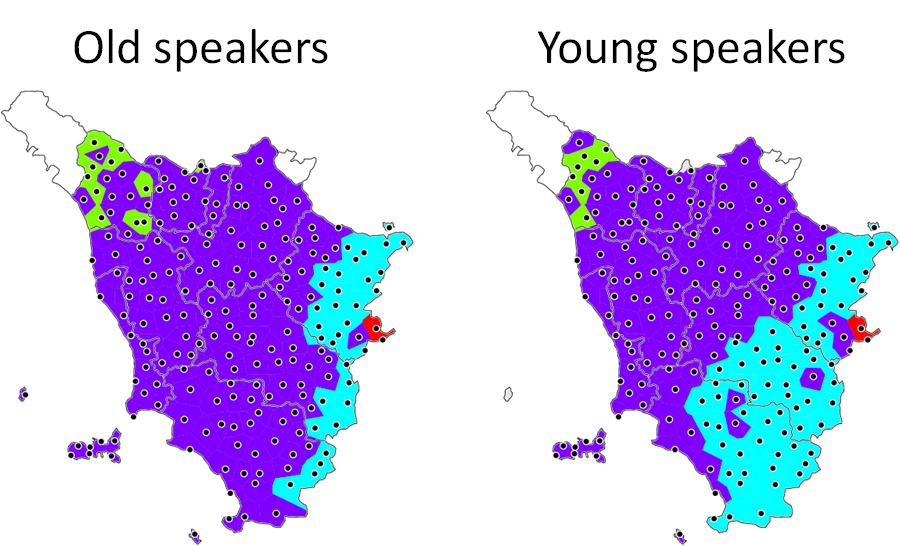
\includegraphics[width=.7\textwidth]{illustrations/monte_wiel_fig4} 
\caption{Geographic visualization of a four-way clustering of \il{Italian!Tuscan}Tuscan varieties on the basis of data from young vs. old speakers.}
\label{fig:monte:4}\is{dialect clustering}
\end{figure}

Besides the different size of the set of associated linguistic features (i.e. more reduced in the case of young speakers), it is interesting to note that 424 salient \isi{lexical features} underlying the old speakers map do not appear among the features underlying the young speakers map. These CL pairs emerging from old speakers correspond typically to old-fashioned and traditional notions as well as less common plants and animals. Examples include \textsc{structure for bed warmer}{}-\textit{prète}, \textsc{poppy}{}-\textit{ròsolo}, \textsc{mutton}{}-\textit{bìrro}, \textsc{set of poplars}{}-\textit{alborellàia}. These CL pairs can be seen as lexical variants which are no longer being used by younger speakers, and these are likely to disappear altogether. 

The number of CL pairs restricted to young speakers is much lower (112) than the number of CL pairs restricted to the old speakers. In this case, the CL pairs correspond to standard Italian words (e.g., \textsc{closet}{}-\textit{ripostìglio}, \textsc{weeping willow}{}-\textit{sàlice piangènte}, \textsc{harvest}{}-\textit{mietitùra}), generic terms (e.g., \textsc{afternoon}{}-\textit{dópo mangiàto}, \textsc{slug}{}-\textit{lumàca ignùda}) or “distorted” (i.e. deviant with respect to traditional pronunciation) variants of dialectal terms (e.g., \textsc{\il{Italian!Tuscan}Tuscan cold cut from pork shoulder}{}-\textit{capricòllo}). The typology of these lexical variants shows the dynamics of \isi{lexical change} ongoing in younger \il{Italian!Tuscan}Tuscan generations, characterized by the loss of local features in favor of generic or standard terms, and by the creative distortion of dialectal words. 

In both cases, however, these CL pairs are not highly ranked (i.e. not the most important) for the associated old and young clusters. Instead, the CL pairs underlying both maps (a total of 769) show clear differences with respect to their ranking. For example, the 1st, 10th, 20th and 50th lexical variants in the ranked list of CL pairs underlying the old speakers map correspond to the 60th, 809th, 59th and 818th position in the young CL pairs list, respectively. Similarly, the 1st, 10th, 20th and 50th ranked lexical variants of the young speakers are ranked (respectively) in the 100th, 13th, 17th and 69th position in the old speakers list. The asymmetry between the old-young vs. young-old correspondences can be seen as the result of a dialect leveling process, causing the lower \isi{importance} of old-fashioned lexical variants for the young speakers (which are top-ranked for the old speaker). Seen from the perspective of young speakers, the disalignment of the ranking is more reduced, reflecting an additional shared set of dialectal lexical items.

\tabref{tab:monte:5} reports the five topmost CL pairs underlying the blue cluster in the two maps. Clearly, the importance values associated with the blue cluster of the old speakers are higher than those associated with the blue cluster of the young speakers. This pattern is confirmed by comparing the average \isi{importance} scores of the top-10 and top-100 CL pairs in the two lists, which are much higher for the old speakers (0.42 vs. 0.34 for the top-10 and 0.26 vs. 0.17 for the top-100). This may also be seen as evidence in support of dialect leveling: lexical areas\is{lexical area} inferred from young speakers data are characterized by less distinctive and/or representative features. 

\begin{table}
\resizebox{\textwidth}{!}{
\begin{tabular}{p{1.5cm}lrrr}
\lsptoprule
{ Cluster} & { Concept-Lexicalization pair} &  { Representativeness} &  { Distinctiveness} &  { Importance}\\
\midrule
\multirow{2}{1.5cm}{Old speakers: Blue cluster} & \textstyleBookTitle{\textsc{grape}}{}-\emph{chìcco} &  0.721 &  0.828 &  0.597\\
& \textstyleBookTitle{\textsc{chestnut}}\textstyleBookTitle{ }\textstyleBookTitle{\textsc{husk}}{}-\emph{rìccio} &  0.706 &  0.661 &  0.467\\
& \textstyleBookTitle{\textsc{embers}}{}-\emph{bràce} &  0.673 &  0.632 &  0.425\\
& \textstyleBookTitle{\textsc{brazier}}{}-\emph{bracière} &  0.596 &  0.680 &  0.405\\
& \textstyleBookTitle{\textsc{hazelnut}}{}-\emph{nocciòla} &  0.794 &  0.507 &  0.403\\
\midrule
\multirow{2}{1.5cm}{Young speakers: Blue cluster} & \textstyleBookTitle{\textsc{bat}}{}-\emph{pipistrèllo} &  0.736 &  0.538 &  0.396\\
& \textstyleBookTitle{\textsc{breast}}{}-\emph{pùppa} &  0.428 &  0.900 &  0.385\\
& \textstyleBookTitle{\textsc{thimble}}{}-\emph{anèllo} &  0.394 &  0.893 &  0.352\\
& \textstyleBookTitle{\textsc{oil}}\textstyleBookTitle{ }\textstyleBookTitle{\textsc{jar}}{}-\emph{cóppo} &  0.437 &  0.772 &  0.337\\
& \textstyleBookTitle{\textsc{eye}}\textstyleBookTitle{ }\textstyleBookTitle{\textsc{gum}}{}-\emph{cìspia} &  0.431 &  0.779 &  0.335\\
\lspbottomrule
\end{tabular}
}
\caption{The five topmost lexical variants of the blue cluster in the young vs. old speakers maps of \il{Italian!Tuscan}Tuscan dialects.}
\label{tab:monte:5}
\end{table}

\section{Conclusion}
In this paper, we illustrated the application of hierarchical spectral partitioning of bipartite graphs in the study of lexical variation in Tuscany based on the dialectal corpus of the \textit{Atlante Lessicale Toscano}. Our results demonstrate the potential of the method in bridging the gap between models of linguistic variation based on aggregate analyses and more traditional analyses based on individual linguistic features. 

By using the HBSGP method, we not only identified existing patterns of lexical variation in Tuscany on the basis of the whole dialectal corpus, but also uncovered the underlying \isi{lexical features} in terms of the characterizing concept-lexicalization pairs\is{concept-lexicalization pair}. The most relevant CL pairs represent the features used to classify and define each identified \isi{lexical area}. To put it in more traditional terms, they can be seen as a proxy of lexical isoglosses\is{isogloss} marking both the qualitative and quantitative distribution of the lexical variants identified as discriminating features of a given lexical dialect area. This entails that the set of the topmost CL pairs associated with each identified lexical dialect area acts as a proxy of bundles of isoglosses\is{bundle of isoglosses}, where the grading of individual isoglosses within the bundle is determined on the basis of the combination of \isi{representativeness} and \isi{distinctiveness}. If the \isi{representativeness} score associated with identified isoglosses (CL pairs) can help to shed light on how much variation exists within the area defined by a given isogloss\is{isogloss}, the distinctiveness score reflects how strongly the lexical variant is concentrated within that area. By comparing the results obtained for different dialect areas, we have seen that different stages of the process of dialect differentiation can be inferred from the different values of these two measures: dialectal subdivisions range from clearly defined areas to areas characterized by fuzzy borders. 

We also investigated whether and to what extent patterns of \isi{lexical variation} and their associated features varied with respect to the granularity\is{granularity of dialectal areas} of the identified dialectal areas and with the age of informants, revealing interesting results. The possibility of exploring linguistic variation at different levels of granularity makes it possible to customize the analysis with respect to the user’s needs. The linguistic features associated with increasingly smaller areas can be seen as \isi{nested isoglosses}, occurring when the spatial distribution of one feature is contained entirely within that of another and establishing an implicational relationship between the two. 

The analysis and comparison of \isi{lexical variation} patterns and associated features across generations showed that the method can also be usefully exploited to track the change in the typology of features in young vs. old informants and to monitor the vitality of a dialect in a given area. In particular, the HBSGP method turned out to effectively capture the dynamics of \isi{lexical change} in Tuscany, by highlighting the emergence of lexical innovations and the obsolescence of old-fashioned traditional dialectal words. 

Current directions of research include testing the robustness of these results by noisy clustering\is{dialect clustering} and the analysis of lexical variation patterns across semantic domains.

\section*{Acknowledgements}
The research reported in this article was carried out in  the framework  of  a  Short  Term  Mobility  program   of international   exchanges   funded   by   the National Council of Research (CNR, Italy). The authors thank the anonymous reviewers for their comments,  which  have  helped  to  improve  this  article.


\printbibliography[heading=subbibliography,notkeyword=this]
\end{document}